\chapter{Systèmes d'exploitation}

	\section{Qu'est-ce qu'un système d'exploitation ?}
	
	\floatpictureright{0.2}{ch-sysex/img/sysex.png}{
		Un système d'exploitation (\textit{Operating System} en anglais, abrégé OS) est un ensemble de programmes. Il a plusieurs fonctions :
		\begin{itemize}
			\item 	c'est un intermédiaire entre l'utilisateur et les applications qu'il utilise (qui sont aussi des programmes) et le matériel ;
			\item 	c'est lui qui partage les \textit{ressources} entre les différents programmes en train d'être exécutés voire entre les différents utilisateurs ;
			\item 	c'est lui qui protège la machine des applications, et les applications les unes des autres ;
			\item 	c'est lui qui gère l'adaptation entre l'\textit{interface} (graphique par exemple) et le matériel.
		\end{itemize}
	}\medskip\par
	Les ressources, ce sont entre autres : 
	\begin{itemize}
		\item 	le matériel qui compose l'ordinateur proprement dit (CPU, mémoire, carte graphique...) et les \textit{périphériques} (imprimante, clé usb, clavier) ;
		\item 	les fichiers ;
		\item 	les éventuelles connexions à des réseaux.
	\end{itemize}
	\floatpictureleft{0.5}
	{img/oss.png}
	{
		Il existe de multiples OS.
		\begin{itemize}
			\item 	pour PC : \textsc{Windows} et beaucoup de distributions de \textsc{Linux} ;
			\item 	pour \textsc{Apple} : \textsc{MacOS} ;
			\item	pour iPhone et iPad : \textsc{iOS} ;
			\item 	pour beaucoup de smartphones : \textsc{Android}.
		\end{itemize}}\medskip\par
	
%---------------

	Les appareils connectés ainsi que les \og box \fg{} des fournisseurs d'accès à Internet et les consoles de jeux disposent aussi de leurs OS.
	Certains OS sont \textit{gratuits}, d'autres \textit{payants}.
	
	\section{Le système de gestion des fichiers}
	
	Un \textit{fichier} est un ensemble de données numériques réunies sous un même nom et enregistré sur un support de mémoire permanent appelé \textit{mémoire de masse} (ce peut être un disque dur, un DVD-rom, une clé USB, une carte SD).\\
	Un \textit{système de gestion de fichiers} est une façon de stocker les fichiers sur la mémoire de masse. La plupart des systèmes d'exploitation stockent les fichiers dans des \textit{répertoires} organisés de manière hiérarchique selon une \textit{arborescence} (voir plus bas).

	\section{L'exemple de Linux et du shell}

	\floatpicturerightcaption{0.5}{ch-sysex/img/pi4.jpg}{les Raspberry Pi tournent sous Linux}{
		En 1970 nait \textsc{UNIX}, l'un des premiers système d'exploitation multi-utilisateurs.\\
		Cependant ce système d'exploitation n'est pas \textit{libre}, c'est à dire que son code source n'est pas à la disposition du public.\\
		En 1991, un étudiant finlandais du nom de Linus Torvalds entreprend de créer un clone d'\textsc{UNIX} en le réécrivant totalement.
	}\medskip\par
	Ce nouveau système d'exploitation libre s'appelle \textsc{Linux} et est désormais largement utilisé.\\
	C'est la plupart du temps une version (appelée \textit{distribution}) de \textsc{Linux} que l'on installe sur les ordinateurs Raspberry Pi.
	
	\begin{center}
		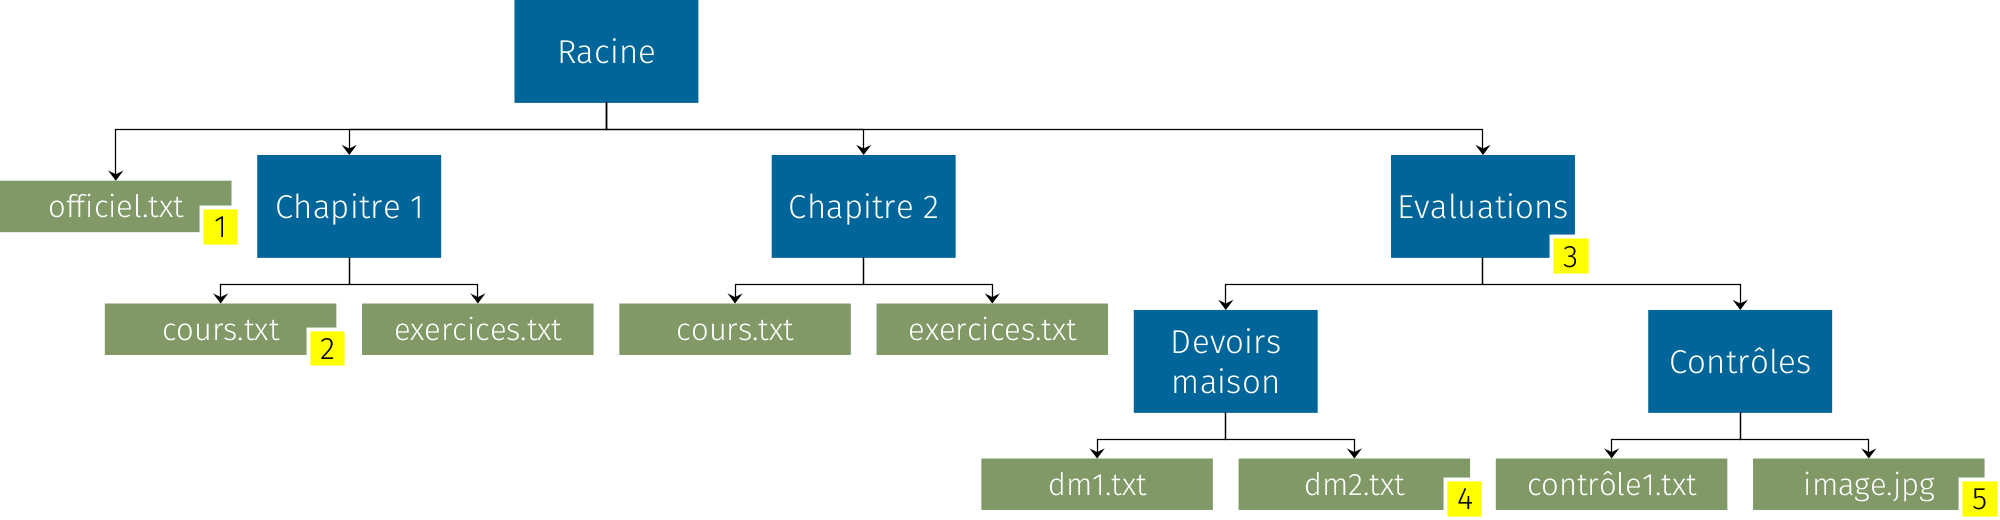
\includegraphics[width=\textwidth]{ch-sysex/img/hier.png}\\
		\footnotesize\textit{Exemple d'arborescence de fichiers.}
	\end{center}

	Dans un système de fichier tel que celui de \textsc{Linux}, la racine se note \texttt{/} et les séparateurs (équivalents des flèches du graphique ci-dessus) aussi.\\
	Il y a deux manières d'accéder aux fichiers.
	\subsubsection{Chemin absolu}
	On part de la racine et on écrit le chemin pour arriver à l'objet désiré.\\
	Ainsi le chemin absolu de l'objet 1 est \texttt{/programme officiel.txt} et celui de l'objet 5 est \texttt{/Evaluations/Contrôles/image.jpg}
	
	\begin{exercice}[]
		Donner les chemins absolus des autres objets.
	\end{exercice}

	

	\subsubsection{Chemin relatif}
	On part d'un emplacement précis (à l'intérieur d'un répertoire) et l'on indique le chemin pour aller à l'objet voulu. S'il faut remonter d'un cran dans l'arborescence on utilise na notation \texttt{..} comme ceci :
	\begin{itemize}
		\item 	si l'on est dans le répertoire \texttt{Evaluations} et qu'on veut accéder à \texttt{dm2.txt} alors son chemin relatif est \texttt{Devoirs maison/dm2.txt};
		\item 	si l'on est dans \texttt{Contrôles} et qu'on veut accéder à \texttt{ch1-exercices.txt} alors son chemin relatif est \texttt{../../Chapitre 1/ch1-exercices.txt} car il faut d'abord remonter l'arborescence de 2 crans.
	\end{itemize}

	\begin{exercice}[]
		On est dans le répertoire \texttt{Contrôles}, donner les chemins relatifs des objets 1 à 5.
	\end{exercice}
	
	\subsection{Le shell}
	
	Nous sommes habitués à un environnement graphique pour gérer les copies et déplacements de nos dossiers (et bien d'autre choses comme par exemple sélectionner des fichiers à compresser) mais ce n'est pas la seule manière. Dans tout système d'exploitation muni d'un environnement graphique, on peut trouver un \textit{terminal} (aussi appelé \textit{invite de commande}, ou \textit{shell}) parce que
	\begin{itemize}
		\item 	c'est avec cette interface textuelle minimaliste que l'on interagissait avec l'\textsc{OS} avant;
		\item 	finalement quand on sait (très bien) s'en servir, on peut faire beaucoup plus de choses plus rapidement avec un shell et au clavier qu'avec un clavier, une souris et un environnement graphique.
	\end{itemize}

	\begin{exercice}[]
		Faire le début de l'activité \og utiliser le shell\fg{} de M. Quinson.

	\end{exercice}
	